\chapter{Releases that change over time}\label{ch:change}

Every floor this book reports for the credit register was computed on a register that does
not move. A loan's exposure is the same in every vintage in which it appears, and whether
it appears is drawn afresh each month, independently of everything else (Chapter~23). A
reader may well take that simplification to be on the safe side. Real exposures amortise, are
drawn down and are restructured; loans close, reopen and are refinanced. To an adversary
who has read a loan's exposure once, every later movement puts distance between what he
holds and what the register publishes, much as the measurement error of Chapter~2 does.
On this view a frozen register hands the adversary the easiest possible target, a value that
waits for him, and an assessment made on it overstates the risk of the register that actually
changes. The view has the shape of a sound rule of thumb: when in doubt, assume the
adversary's task is easy.

The view fails on the extension's evidence run. On a synthetic panel of 3,000 loans in 12
key classes, an adversary who knows a loan's history of activity and holds a noisy reading of
its exposure in each vintage it is live identifies 403 of 1,200 targets after six vintages when the
panel is frozen, a rate of $0.336$ with an exact upper bound of $0.359$. On the same panel with
exposures that drift and activity that persists, the same adversary identifies 703 of 1,200, a
rate of $0.586$ with an upper bound of $0.610$. The frozen panel understates what the changing
one reveals by 300 of the 1,200 targets.
% source: draft 2, Table 19.1 (six-vintage row)

At the Bank, the question came from two directions in the same week. Tom\'as's second
file would extend his history from six vintages to twelve (Chapter~\ref{ch:learning}), and the chair asked whether the certificate for the first file could simply be read forward. The supervision department, for its part, argued that the register's exposures move every month, so any figure
computed on a frozen stand-in must overstate the risk, and the floor of 75 could safely be
lowered for monthly files. Naledi did not know which side was right. She knew only that
the old certificate had assumed the register stood still.

This chapter asks one question: what does an adversary learn from a register whose exposures
and activity change over time, and can a frozen register stand in for it? It begins by fixing what
is being measured, because a register that changes offers more than one denominator. It
then shows that the naive way of combining several readings overstates the evidence they
carry, sets out the extension's model of changing exposure and activity, measures the pooled
attack on it, and describes a simpler graph model that any richer model of change must beat.
It ends with what the evidence does not yet show.

\section{One experiment, one denominator}

A risk figure changes meaning whenever the target population, the auxiliary information,
the attack or the conditioning changes, and a register that changes over time multiplies
the ways in which these can drift apart. The objects are those of Chapter~2. Let $D$ be the
confidential register, $Y_\theta$ the release under setting $\theta$, $J$ the target's released identity with $J=0$
for no match, $I$ the set of released candidates and $S=\ind{J\in I}$ the event of membership.
The adversary observes $O=(Z,Y_\theta)$ with background information $B_a$, and the attack $\delta_a(O)$
names an element of $I$ or abstains. For a fixed target, the unconditional and membership-conditional risks of Definition~2.1 are related by (2.3), $R^{\rm unc}=\pi R^{\rm in}$ with $\pi=\Prob(S=1\mid t,B_a)$, and no independence is needed for that. A sampling fraction may stand in for $\pi$ only when
conditioning on $B_a$ leaves it unchanged; an adversary who knows that the target is in the
file has $\pi=1$ whatever the sampling fraction.

Population risk needs a declared law over targets. With weights $w_t\ge0$ summing to one,
$r_a(\theta)=\sum_t w_t R^{\rm unc}_a(t,\theta)$. Averaging over released targets only defines a different law and
must be named as such. On a credit register there are at least three natural laws, and they
are not interchangeable: an average over borrowers, an average over loans, and an average
weighted by lender. A borrower with five loans counts once under the first and five times
under the second.

The correction of Chapter~2 belongs here too. A forced-choice attack that names the most
probable released candidate succeeds, given the observations and membership, with probability $\max_{j\in I}p_j/(1-p_0)$, where $p_0$ is the posterior on no match (equation~(2.6) and Proposition~2.4).
An earlier draft of that equation left out the denominator, and the book's figures were unaffected because its simulated attacks normalise over released candidates only. A model
of change does not alter the correction. It does make the no-match term harder to ignore,
because in a changing register a target can be absent from one vintage and present in the
next.

That last point fixes the denominator for the experiments in this chapter. The extension's
run draws its targets from loans that are live in the first vintage, takes the first 400 such loans
in each of three synthetic panels, and counts success over all 1,200 of them. Membership is
conditioned on at the first vintage only. A target's absence from a later vintage is not a
reason to drop it from the denominator: it is a published fact the adversary can use. An
assessment that conditioned on presence in every vintage would remove from the count
exactly the targets whose pattern of absences makes them easiest to find.

Naledi wrote this into the plan for the twelve-vintage file before she ran anything. The
target law was over loans, since Tom\'as's study was of lending relationships; the conditioning was on presence in the first month of the new file; and absence later was part of what the
adversary saw. Grace, reading the draft plan, asked what happened to a loan that closed in
the third month. Naledi's answer was that it stayed in the denominator and that its closure
was part of the attack.

\section{Many readings are not many independent pieces of evidence}

An adversary who holds several readings of a target, one for each vintage or each auxiliary
source, has to combine them. The simplest combination multiplies the likelihoods of the
readings, as naive Bayes does, and as the record-linkage weights of \citet{fellegi1969} do
when they add the evidence of each agreeing field:
\begin{equation}\label{c19:eq-naive}
L_j(z)=\prod_{h=1}^{m}p(z_h\mid J=j).
\end{equation}
This assumes the readings are independent given the identity of the target. It does not
assume they are independent in the population, which is a different and weaker statement.
The assumption fails whenever readings share an error: when one stale figure is copied
into several months, when two auxiliary sources took their numbers from the same filing,
or when an exposure is reported twice under two loan identifiers. A Gaussian model with
covariance $\Sigma$ keeps the shared error in view:
\begin{equation}\label{c19:eq-gauss}
\log L_j(z)=-\tfrac12(z-\mu_j)^\top\Sigma^{-1}(z-\mu_j)-\tfrac12\log|\Sigma|-\tfrac m2\log(2\pi).
\end{equation}
The off-diagonal entries of $\Sigma$ carry the point. Ten identical readings are one reading written ten times. A classifier built on \eqref{c19:eq-naive} can still name the right candidate when the readings share errors, but the probabilities it reports are then unreliable \citep{domingos1997}, and a risk assessment reads those probabilities.

\begin{proposition}[Correlated readings and naive evidence]\label{c19:prop-corr}
Let $z\in\mathbb R^m$ be readings with $z\mid J=j\sim N(\mu_j\mathbf 1,\Sigma)$, where $\Sigma=\sigma^2[(1-\rho)I+\rho\mathbf 1\mathbf 1^\top]$ with $\sigma>0$ and $0\le\rho<1$. For two
candidates with $\mu_j-\mu_k=\Delta$, the expected log-likelihood ratio in favour of the true candidate $j$ is
\begin{equation}\label{c19:eq-llr}
\E\Big[\log\frac{L_j(z)}{L_k(z)}\,\Big|\,J=j\Big]=\frac{\Delta^2}{2\sigma^2}\cdot\frac{m}{1+(m-1)\rho}
\end{equation}
under the correct model \eqref{c19:eq-gauss}, and $m\Delta^2/(2\sigma^2)$ under the naive model \eqref{c19:eq-naive} with independent
errors of variance $\sigma^2$. The naive figure is larger by the factor $1+(m-1)\rho$. As $m$ grows the correct
figure tends to $\Delta^2/(2\sigma^2\rho)$ for $\rho>0$, while the naive one grows without bound.
\end{proposition}

The expected log-likelihood ratio is the evidence a typical reading set carries against
the wrong candidate, and posterior odds move by its exponential. With a correlation of
one half, twenty readings carry the evidence of fewer than two independent ones, and a
naive posterior built on them is overconfident by a factor in the exponent of more than
ten. The size of the overstatement depends on how the figure is computed. An assessment that reports the expected
maximum posterior from a naive model overstates the adversary's confidence. A simulation
that draws the adversary's reading errors independently, when the real adversary's errors
are shared, credits the simulated adversary with more information than the real one has.
Both errors lie on the side of overstating risk, but neither is a measurement, and the second
is an assumption about the adversary that ought to be written down.

The extension's run makes that assumption. Its adversary receives a fresh, independent
reading error in every vintage in which the target is live, with standard deviation $0.3$ on
the log scale. On a frozen panel those are several independent readings of one unchanging
value, and their average has a standard deviation smaller by the square root of their number.
On a changing panel each reading is of a different value, and the readings carry the path of
the exposure as well as its level. That difference drives much of what follows.

Naledi asked herself which adversaries at the Bank would hold readings of each kind.
Pieter reads his own bank's books, which record each month's exposure as it stands, so his
readings follow the path and his errors are small and unshared. An outsider who copies
a figure from a firm's annual report into each month has one reading with a shared error,
repeated. She declared the two separately. For the outsider she counted the twelve months
as one reading, which is what the proposition gives as $\rho$ approaches one, since the engine's
attack draws independent errors and would have credited him with twelve.

\section{A model of changing exposure and activity}

The extension proposes a first model for the two features that Chapter~23 left open: exposures
that change between vintages, and activity that depends on the past. For loan $j$ in
vintage $t$, let $e_{j,t}$ be its exposure and $a_{j,t}\in\{0,1\}$ its activity. Log exposure follows a first-order autoregression around a long-run level $\bar e$, the simplest of the dynamic panel models of
econometrics \citep{arellano1991},
\begin{equation}\label{c19:eq-ar}
\log e_{j,t+1}-\bar e=\mu+\varphi(\log e_{j,t}-\bar e)+\epsilon_{j,t},\qquad\epsilon_{j,t}\sim N(0,\sigma^2),\quad|\varphi|<1,
\end{equation}
and activity follows a logistic transition, a Markov regression of the kind \citet{zeger1988} set out for binary series,
\begin{equation}\label{c19:eq-act}
\Prob(a_{j,t+1}=1\mid a_{j,t},e_{j,t})=\operatorname{logit}^{-1}\!\big(\gamma_0+\gamma_1a_{j,t}+\gamma_2(\log e_{j,t}-\bar e)\big).
\end{equation}
The extension also allows borrower characteristics $x_j$ in \eqref{c19:eq-act}; the engine's version omits
them.

Two choices in this model need stating. First, $e_{j,t}$ is defined while a loan is inactive,
as a latent potential exposure: the amount the loan would carry if it were live. Without
that convention the autoregression has nothing to evolve during an inactive spell, and the
model would have to specify origination and closure as separate processes. Second, the
pooled likelihood of a target's readings integrates over the whole latent path. An attack
that matched each date's marginal distribution separately would discard the dependence
between dates, which is exactly what makes a path identifying.

\begin{example}[Two loans that start together]\label{c19:ex-paths}
Take two loans in Pieter's key class, both
live, both with log exposure $11.60$ (about 109,000) in the first vintage. The numbers are
illustrative. Let $\bar e=11$, $\mu=0$ and $\varphi=0.95$, as in the run's changing setting, and suppose
the first loan draws shocks of $+0.10$ and $-0.20$ in the next two months and the second draws
$-0.10$ and $+0.15$. By \eqref{c19:eq-ar} the first loan's path is $11.60\to11+0.95\times0.60+0.10=11.67\to11+0.95\times0.67-0.20=11.44$, and the second's is $11.60\to11.47\to11.60$. Pieter's
target is the first loan, and suppose his three readings fall exactly on its path. The engine's
attack scores each candidate by $-\tfrac12\sum_t(\text{published}_t-\text{reading}_t)^2/0.3^2$. The first loan scores 0. The
second differs by 0, $0.20$ and $0.16$ and scores $-\tfrac12(0.20^2+0.16^2)/0.09=-0.364$, so the first
loan is $e^{0.364}=1.44$ times as likely, and between the two the attack gives it probability $0.59$.
On a frozen panel both loans would publish $11.60$ in every month, the scores would tie, and
the attack could do no better than a coin toss. Each month of movement adds a term in
which the loans differ. Two months moved the odds from even to $1.44$; a year of movement
would add ten more such terms.
\end{example}

With $\varphi=1$, $\sigma=0$ and $\gamma_1=\gamma_2=0$ the model reduces to a frozen panel: exposure never
changes, and each loan is live in each vintage with probability $\operatorname{logit}^{-1}(\gamma_0)$, independently
of its past and its size. The engine's frozen setting takes $\gamma_0=2$, so a loan is live with
probability about $0.88$ in each vintage after the first. The changing setting of the run takes
$\varphi=0.95$, $\sigma=0.15$, $\gamma_0=0$, $\gamma_1=1.5$ and $\gamma_2=0$: a live loan stays live with probability about
$0.82$, an inactive one returns with probability one half, and across the six vintages 79 per
cent of loan-months are live. Every loan is live in the first vintage, log exposure starts from
a normal law with mean 11 and standard deviation $1.2$, and each loan's key class is drawn
uniformly from twelve.

These are chosen parameters, not estimates, and two of them bite. With $\gamma_2=0$, activity
in the run does not depend on exposure, so the dependence of activity on loan size that
Chapter~23 named is in the model and not in the evidence. And the frozen limit is not the
register of Chapter~\ref{ch:credit}. That register was rebuilt after review, with originations during the
panel, a monthly exit hazard of $0.04$ with no return and a stock of about 27,000 loans. The
extension's panel forces every loan to be live in the first vintage and lets loans vanish and
return, which is the design the referees criticised. Its frozen rows are a reference for this
panel only, and they should not be compared with the floors of Table~13.4.

\section{The pooled attack, using presence and absence}

The engine's pooled attack runs three adversaries on each panel. All three know the target's
key class and that its loan is live in the first vintage. The first knows nothing else and chooses
at random among the loans of the class. The second also knows the target's activity in every
pooled vintage, and strikes out every candidate whose pattern of presence and absence
differs. The third knows the history and holds, for each vintage in which the target is live,
a reading of its log exposure with error of standard deviation $0.3$; it scores the remaining
candidates by the Gaussian likelihood of those readings and names the most likely one. A
candidate that is absent in a vintage where the target is live offers no published value to
compare, and the attack rules it out. Absence is information. The first published version of
the history attack had used only presence, and the referees pointed out that an adversary
who knows when a loan is live also knows when it is not (Chapter~23).

The history adversary can be analysed exactly, and the analysis explains its rows in the
evidence.

\begin{proposition}[Success from activity patterns]\label{c19:prop-pattern}
Let a key class hold $n$ loans, all live in the first
vintage, whose activity patterns over vintages $2,\dots,v$ are independent across loans with a common
law $P$ on the set $\Pi_v$ of possible patterns. An adversary who knows the target's key and pattern and
names a loan chosen uniformly among those in the class with the same pattern identifies a target
drawn uniformly from the class with probability
\begin{equation}\label{c19:eq-s}
s_v=\frac1n\sum_{\pi\in\Pi_v}\big[1-(1-P(\pi))^n\big]=\frac{\E[\text{number of distinct patterns among the }n\text{ loans}]}{n}.
\end{equation}
Consequently $s_v\le\min(1,2^{v-1}/n)$, and $s_v$ never decreases as $v$ grows.
\end{proposition}

The proposition turns the history attack into a count. The adversary succeeds as often
as the class contains distinct patterns, divided by its size. A frozen panel whose loans are
live nine months in ten produces few distinct patterns, because most loans show the same
unbroken run. A panel in which loans persist when live and stay away for a while when not
spreads its loans over more patterns, and the adversary does better.

\begin{example}[Counting patterns in a class of four]\label{c19:ex-count}
Naledi checked the proposition on the
smallest case she could hold in her head: a key class of four loans and three vintages, so
that each loan shows one of four patterns over the second and third months. On the frozen
panel each later month is live with probability $\operatorname{logit}^{-1}(2)=0.881$, independently, and the
four patterns have probabilities $0.776$ (live, live), $0.105$ (live, absent), $0.105$ (absent, live) and
$0.014$ (absent, absent). On the changing panel a live loan stays live with probability $0.818$
and an absent one returns with probability one half, which gives $0.668$, $0.149$, $0.091$ and $0.091$.
Equation~\eqref{c19:eq-s} sums $1-(1-P(\pi))^4$ over the patterns: the expected number of distinct
patterns is $1.77$ on the frozen panel and $2.10$ on the changing one, and the history adversary
succeeds with probability $1.77/4=0.44$ and $2.10/4=0.52$. The key-only adversary, who
picks among the four at random, succeeds with probability $0.25$. Simulating 20,000 such
classes with the engine's panel and attack gave $0.443$ and $0.522$. The changing panel spreads
its loans more evenly over the patterns, and evenness is what the adversary needs.
\end{example}

\begin{table}[ht]
\centering\small
\caption{Pooled attacks on the extension's synthetic panels: successes out of 1,200 targets (400
in each of three panels of 3,000 loans in 12 key classes), with the exact one-sided 95 per cent upper
bound in brackets. The key-only adversary does not use the vintages and is the same for both panels.
Readings have standard deviation $0.3$ on the log scale. All figures are synthetic.}
\label{c19:tab-pooled}
\begin{tabular}{c l ll ll}
\toprule
 & & \multicolumn{2}{c}{Frozen panel} & \multicolumn{2}{c}{Changing panel}\\
\cmidrule(lr){3-4}\cmidrule(lr){5-6}
Vintages & Key only & History & History and readings & History & History and readings\\
\midrule
1 & 3 (0.006) & 3 (0.006) & 39 (0.042) & 3 (0.006) & 39 (0.042)\\
2 & 2 (0.005) & 7 (0.011) & 96 (0.094) & 7 (0.011) & 96 (0.094)\\
3 & 2 (0.005) & 20 (0.024) & 143 (0.136) & 17 (0.021) & 200 (0.185)\\
4 & 3 (0.006) & 25 (0.029) & 245 (0.224) & 33 (0.037) & 378 (0.338)\\
5 & 5 (0.009) & 56 (0.058) & 319 (0.288) & 81 (0.081) & 541 (0.475)\\
6 & 7 (0.011) & 90 (0.089) & 403 (0.359) & 134 (0.128) & 703 (0.610)\\
\bottomrule
\end{tabular}
% source: draft 2, Table 19.1
\end{table}

At six vintages there are at most 32 patterns, so in a class of 250 loans, the average size
in a panel of 3,000 loans and 12 classes, the history adversary cannot exceed about $0.13$.
Evaluated at the run's parameters, \eqref{c19:eq-s} reproduces the history rows of the evidence for
both panels to within their sampling error.

Table~\ref{c19:tab-pooled} gives the full evidence, and Figure~\ref{c19:fig-pooled} draws its two informative columns.
Read the key-only column first, because it is a check. That adversary does not use the vintages, so its success should stay near one in 250 whatever the number pooled, and it does:
between 2 and 7 successes in 1,200 for both panels. The first vintage is identical for both
panels by construction, since nothing has yet changed. At two vintages the two panels give
the same totals, 7 for the history adversary and 96 with readings. One transition offers only
two patterns in either panel, and \eqref{c19:eq-s} gives nearly the same value for both, so the history
adversary is expected to do about equally well; the equal readings totals are partly chance,
since the counts differ panel by panel and happen to sum alike. From three vintages on the
panels separate, and the gap widens with every vintage. At six the history adversary succeeds for $0.075$ on the frozen panel and $0.112$ on the changing one, and the adversary with
readings for $0.336$ and $0.586$.

\begin{figure}[ht]
\centering
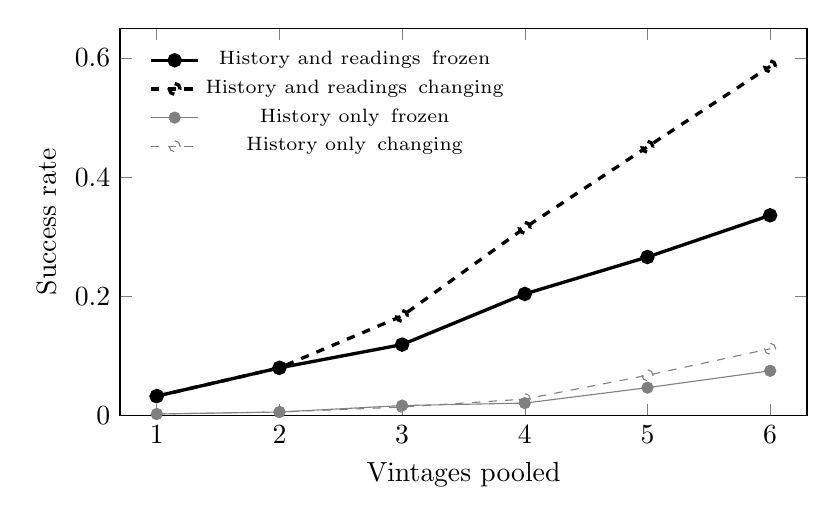
\begin{tikzpicture}
\begin{axis}[width=0.85\textwidth,height=6.5cm,xlabel={Vintages pooled},ylabel={Success rate},
  xmin=0.7,xmax=6.3,ymin=0,ymax=0.65,xtick={1,2,3,4,5,6},
  legend style={at={(0.03,0.97)},anchor=north west,draw=none,font=\scriptsize,fill=white}]
\addplot[black,very thick,mark=*] coordinates {(1,0.0325) (2,0.08) (3,0.119) (4,0.204) (5,0.266) (6,0.336)};
\addplot[black,very thick,dashed,mark=o] coordinates {(1,0.0325) (2,0.08) (3,0.167) (4,0.315) (5,0.451) (6,0.586)};
\addplot[gray,thin,mark=*] coordinates {(1,0.0025) (2,0.0058) (3,0.0167) (4,0.0208) (5,0.0467) (6,0.075)};
\addplot[gray,thin,dashed,mark=o] coordinates {(1,0.0025) (2,0.0058) (3,0.0142) (4,0.0275) (5,0.0675) (6,0.112)};
\legend{History and readings\, frozen,History and readings\, changing,History only\, frozen,History only\, changing}
\end{axis}
\end{tikzpicture}
% source: draft 2, Table 19.1 (successes divided by 1,200)
\caption{Success of the pooled attack against the number of vintages pooled, on the extension's
synthetic panels. Solid lines with filled marks are the frozen panel; dashed lines with open marks
are the changing panel. Heavy black lines are the adversary with history and a reading in each live
vintage; thin grey lines are the adversary with history only. Each point is a rate over 1,200 targets;
the counts and upper bounds are in Table~\ref{c19:tab-pooled}.}
\label{c19:fig-pooled}
\end{figure}

Two mechanisms produce the gap, and the proposition and the readings section each
account for one. The changing panel spreads loans over more activity patterns, so the history
alone leaves fewer candidates. And on the changing panel each vintage's reading is of a new
value along which candidates differ, so the readings accumulate evidence about a path; on
the frozen panel they only refine one number. The run cannot say how much of the gap
each mechanism explains, because the changing setting alters both at once: activity is less
frequent and more persistent, and exposure moves. A run that varied them one at a time
would split the gap. It has not been done.

The misconception treated change as noise in the adversary's information. That holds for
an adversary whose information is stale, one who read a loan's exposure once and compares
that reading with later published values. For him a moving exposure does blur the match,
and a frozen register overstates his success. It fails for an adversary who observes the target
as it changes, a lender, a counterparty or anyone with a monthly source, because for him
change is signal: it gives the target a path that no other loan shares. A frozen register is
conservative for some adversaries and optimistic for others, and the evidence run shows the
optimism can be large. It cannot be assumed conservative without saying which adversary
is meant. The documented cases point the same way. A few film ratings with rough dates
were enough to pick out subscribers in the Netflix Prize data \citep{narayanan2008}, and four points in space and time singled out 95 per cent of the people in a mobility
data set of 1.5 million \citep{demontjoye2013}. A path is a set of such points.

Naledi took Table~\ref{c19:tab-pooled} to the committee with one sentence above it: the frozen figure
was too low for any adversary who watched the register month by month, and those were
the adversaries the Bank worried about. The supervision department's proposal to lower the
floor for monthly files was withdrawn. The chair's question about reading the old certificate
forward had its answer too: the certificate covered six vintages of a register assumed to stand
still, and the twelve-vintage file had to be audited afresh.

\section{A graph model that has to stay in the comparison}

Changing exposure and activity are one kind of movement. Another is movement between
discrete states: a borrower changes sector, a loan moves between lenders, a firm crosses
a size threshold. The extension's simplest model for that movement is a continuous-time
Markov chain on a graph of states, the model that credit-risk work has long used for movements between rating grades \citep{jarrow1997,lando2002}. Let $c_i(t)$ be
the mass of targets in state $i$, and let $Q$ be a generator: $Q_{ij}\ge0$ for $i\ne j$, and $Q_{ii}=-\sum_{j\ne i}Q_{ij}$.
For masses written as a column vector,
\begin{equation}\label{c19:eq-graph}
\dot c=Q^\top c,\qquad c(t)=\exp(tQ^\top)\,c(0),
\end{equation}
and with a disclosure risk $g_i$ for a target in state $i$, the model risk is $r(t)=g^\top c(t)/\mathbf 1^\top c(t)$.
The engine computes the matrix exponential with SciPy's scaling-and-squaring routine \citep{almohy2009}; \citet{moler2003} review why the naive ways of computing it fail.

\begin{proposition}[The graph baseline]\label{c19:prop-graph}
Let $Q$ be a generator and $c(0)\ge0$. Then:
\begin{enumerate}
\item $c(t)\ge0$ and $\mathbf 1^\top c(t)=\mathbf 1^\top c(0)$ for every $t\ge0$;
\item if $\mathbf 1^\top c(0)>0$, the model risk $r(t)$ lies between the smallest and the largest of the $g_i$;
\item if complete paths are observed, with $n_{ij}$ transitions from $i$ to $j$ and total time $T_i>0$ spent in
state $i$, the maximum-likelihood estimate of $Q_{ij}$ for $j\ne i$ is $n_{ij}/T_i$.
\end{enumerate}
\end{proposition}

The first part is what a model of movement has to get right before anything else: no
state may hold a negative number of targets, and none may be created or lost. The second
says the model risk is an average of state risks, so it can never exceed the riskiest state.
The third says that the rates can be read off transition counts and holding times, with no
optimisation; \citet{albert1962} derived this estimator, and \citet{lando2002} used it
for rating transitions. Together they make the graph model cheap and hard to get wrong,
and those are the reasons it has to stay in any comparison. The extension goes on to propose
continuous transport models and an optional fluid closure, which Chapter~20 examines. A
richer model of movement earns its place only by predicting held-out periods better than
this baseline, or by supplying a structural constraint that has meaning on its own.

\begin{example}[Mass moving across three states]\label{c19:ex-graph}
The supervision department, still interested in movement, asked Naledi what the graph model would say about restructured loans.
She wrote down three illustrative states: performing small loans, performing large loans and
restructured loans, with disclosure risks $g=(0.02,0.05,0.30)$, since restructured loans are
few and stand out. Per year, small loans grow large at rate $0.10$ and are restructured at $0.05$;
large loans shrink at $0.05$ and are restructured at $0.05$; restructured loans return to the small
class at $0.20$. Suppose a sample of paths had shown 6 moves from small to large and 3 to
restructured in 60 loan-years spent small, 2 and 2 in 40 loan-years spent large, and 4 returns
in 20 loan-years spent restructured. Part 3 gives $6/60=0.10$, $3/60=0.05$, $2/40=0.05$
twice and $4/20=0.20$, which is the generator above. Starting from masses $(0.6,0.3,0.1)$,
the model risk is $0.6\times0.02+0.3\times0.05+0.1\times0.30=0.057$. After one year the masses are
$(0.552,0.326,0.122)$ and the risk is $0.064$; after five, $(0.449,0.379,0.171)$ and $0.079$; in the long
run, $(0.4,0.4,0.2)$ and $0.088$. The masses sum to one at every time, and the risk stays below
the largest state risk, $0.30$, as part 2 requires. The risk rises by half without any loan changing what it publishes, only because mass drifts towards the restructured state. Whether the
Bank's loans move at these rates is a question for its own transition counts.
\end{example}

The evidence run checks part 3 on a chain of four states with known rates between $0.05$
and $0.15$. It simulates 400 complete paths over a horizon of 10, counts the transitions and
holding times, and estimates the generator. The largest error in any estimated entry is $0.016$.
Started from masses of $0.4$, $0.3$, $0.2$ and $0.1$ and run forward to time 5, the true and estimated
generators give the masses in Figure~\ref{c19:fig-graph}: $0.202$, $0.360$, $0.220$ and $0.218$ under the true rates,
and $0.198$, $0.369$, $0.215$ and $0.218$ under the estimates. Both sets sum to one. The largest
error in a mass, in the second state, is under $0.01$. The check verifies the estimator on data
generated by the model it assumes. It says nothing yet about whether lenders, sectors or
size classes in a real register move as a Markov chain.

\begin{figure}[ht]
\centering
\begin{tikzpicture}
\begin{axis}[width=0.7\textwidth,height=5.5cm,ybar,bar width=12pt,ylabel={Mass at time 5},ymin=0,ymax=0.45,
  symbolic x coords={State 1,State 2,State 3,State 4},xtick=data,enlarge x limits=0.18,
  legend style={at={(0.97,0.97)},anchor=north east,draw=none,font=\scriptsize,fill=white}]
\addplot[black,fill=gray!45] coordinates {(State 1,0.202) (State 2,0.360) (State 3,0.220) (State 4,0.218)};
\addplot[black,pattern=north east lines] coordinates {(State 1,0.198) (State 2,0.369) (State 3,0.215) (State 4,0.218)};
\legend{True generator,Estimated from 400 paths}
\end{axis}
\end{tikzpicture}
% source: draft 2, Figure 19.2 and the text of Section 19.5
\caption{The graph baseline in the extension's evidence run. Masses in four states at time 5,
starting from $0.4$, $0.3$, $0.2$ and $0.1$, under the true generator (solid grey) and under the generator
estimated from transition counts and holding times on 400 simulated paths (hatched). Synthetic
data.}
\label{c19:fig-graph}
\end{figure}

\section{What the evidence does not show}

Everything in this chapter is synthetic. The panels were generated with chosen parameters,
the readings with a declared error, and the graph with a generator written into the script.
The evidence shows that a changing register can reveal far more than its frozen version to
an adversary who watches it, and that the engine's models behave as their mathematics says.
It does not show how much more a real register reveals.

For the same reason the book's credit-register floors have not been recomputed under
the dynamic model, and the extension's own status table records the step as open. There
are four reasons, and each would have to be removed first. The model's parameters are
chosen, and a floor computed from them would encode those choices while looking like a
measurement. The panel on which the model runs is not the register of Chapter~\ref{ch:credit}: it lacks
originations, irreversible exits, unequal lenders and the key structure of that register, and it
forces every loan to be live at the start. The floors of Chapter~\ref{ch:credit} came from fixed-sequence
selection with confirmation on 4,000 targets per level, and nothing of that kind has been run
on the panel. And the dependence of activity on loan size, the feature that most separates a
real register from the frozen one, was switched off in the run. Replacing chosen parameters
with estimated ones needs a governed register, which is step 10 of the extension's plan, and
validating the result needs step 17.

The direction of the evidence is still useful before its size is known. A floor that was
set on a frozen register should not be lowered on the argument that real exposures move.
If anything, the movement argues for a stricter floor against adversaries who watch the
register, and for auditing each extension of a history afresh.

Grace's note on the twelve-vintage decision was short. The audit had run on the Bank's
own twelve months inside the secure environment, so it already contained whatever movement the register had; the frozen model bore only on the old synthetic certificate, which
the committee had stopped reading forward. She asked for one more thing, and the chair
agreed: that the Bank estimate the autoregression and the activity transition on its own register, inside the secure room, so that the next synthetic assessment could use parameters the
Bank had measured.

\section{The answer}

The chapter asked what an adversary learns from a register whose exposures and activity
change over time, and whether a frozen register can stand in for it. An adversary who
watches the register month by month learns the target's path: its pattern of presence and
absence, and the sequence of its exposures. Change gives each loan a path that others do
not share, so it adds to what this adversary learns. On the extension's synthetic panels, six
vintages of history and readings identify a target $0.34$ of the time when the panel is frozen
and $0.59$ when it changes, and the history alone identifies $0.075$ and $0.112$. A frozen register
is conservative only for an adversary whose information is stale, and it cannot be assumed
conservative without naming the adversary. Measuring the real gap needs a model fitted
to a real register, a target law and conditioning event fixed before the attack runs, readings
whose shared errors are modelled and not multiplied away, and a simple graph baseline that
any richer model of change must beat. Until a governed register supplies the parameters,
the book's floors stand as properties of a frozen synthetic register, and the dynamic model
remains code and tests.

\begin{inpractice}[In practice: assessing a register that changes]
Fix the target law (borrowers, loans or lenders) and the vintage at which membership is
conditioned before running any attack, and keep targets that later disappear in the denominator.
Declare, for each adversary, whether its readings follow the target's path or repeat one stale
value, and model shared errors with a covariance instead of multiplying likelihoods. Run the
pooled attack with presence and absence both used. Do not read a certificate forward to a longer
history; audit the new history. Do not lower a floor because exposures move. When a model of
change is used, report its parameters, say whether they were chosen or estimated, and compare
it with the graph baseline on held-out periods.

\medskip\noindent\textit{In the software.} The panel model and attack are in \texttt{privacy\_risk.dynamics}: \texttt{PanelModel}
(with \texttt{PanelModel.static} for the frozen limit), \texttt{simulate\_panel} and \texttt{pooled\_attack},
which returns integer counts. The graph baseline is in \texttt{privacy\_risk.graph}:
\texttt{validate\_generator}, \texttt{propagate}, \texttt{node\_risk} and \texttt{estimate\_generator}. The membership correction is \texttt{linkage.membership\_success}, and \texttt{linkage.fixed\_target\_success}
counts successes for one fixed target. The tests are in \texttt{tests/test\_ext\_models.py} and
\texttt{tests/test\_ext\_conditioning.py}, and \texttt{scripts/extension\_evidence.py} regenerates Table~\ref{c19:tab-pooled} and Figure~\ref{c19:fig-graph}. Algorithm~19.1 sets out the pooled attack, including its treatment of
absence, and its checks reproduce the six-vintage row of Table~\ref{c19:tab-pooled}. These modules belong to the extension's code bundle and are not in this repository's \texttt{src/privacy\_risk}.
\end{inpractice}

\begin{mdframed}[linecolor=gray!60,backgroundcolor=gray!5]
\textbf{Algorithm 19.1.} The pooled attack, using presence and absence.\par\smallskip
\textit{Input.} A panel of loans over $v$ vintages, each loan $k$ with a key class, an activity $a_{k,t}$ and a log
exposure $\log e_{k,t}$ in each vintage; the number $w$ of vintages pooled; a list of targets; whether the
adversary knows each target's activity; the standard deviation $s$ of its readings of log exposure,
if it holds any; a seeded random source.\par
\textit{Output.} The number of targets the adversary names correctly, and the number of targets.
\begin{enumerate}
\item Refuse the inputs unless $1\le w\le v$, and keep only the first $w$ vintages.
\item For each target $j$, refuse the inputs if $j$ is not live in the first vintage. Otherwise its candidates
are the loans of its key class that are live in the first vintage.
\item If the adversary knows the target's activity, keep only the candidates whose pattern of presence and absence over the $w$ vintages equals the target's in every vintage (Proposition~\ref{c19:prop-pattern}).
\item If the adversary holds readings with $s>0$, draw a reading $y_t=\log e_{j,t}+sZ_t$, with $Z_t$
standard normal, for each vintage $t$ in which the target is live. Score each candidate $k$ by
$-\tfrac12\sum_t(\log e_{k,t}-y_t)^2/s^2$ over those vintages, as in Example~\ref{c19:ex-paths}. A candidate absent in any
of those vintages offers no published value there and takes a residual of $10^6$, which rules it
out. Keep the candidates with the highest score.
\item Name one of the remaining candidates at random, each equally likely, and count a success
if it is the target.
\item Return the number of successes and the number of targets.
\end{enumerate}
\textit{Checks, each run against the software by the test suite:}
\begin{itemize}
\item Changing panel of Table~\ref{c19:tab-pooled}, adversary who knows the history, six vintages, successes summed over the three panels of 400 targets: 134.
\item The same adversary with readings of standard deviation $0.3$: 703.
\item Frozen panel, adversary who knows the history, six vintages: 90.
\item Frozen panel, adversary who knows only the key class, six vintages: 7.
\item Two loans in one class with the same exposures, the other loan absent in the second of three
vintages, an adversary with readings but no activity history, share of 200 tries that succeed: $1.000$.
\item The same pooling only the first vintage, where the two loans cannot be told apart: $0.480$.
\item A target that is not live in the first vintage: refused.
\item Four vintages pooled from a panel of three: refused.
\end{itemize}
\end{mdframed}

\section{Proofs}

\begin{proof}[Proof of Proposition~\ref{c19:prop-corr}]
The vector $\mathbf 1$ is an eigenvector of $\Sigma$: $\Sigma\mathbf 1=\sigma^2[(1-\rho)\mathbf 1+\rho m\mathbf 1]=\sigma^2(1+(m-1)\rho)\mathbf 1$. Since $0\le\rho<1$, every eigenvalue of $\Sigma$ is positive (the others equal
$\sigma^2(1-\rho)$), so $\Sigma$ is invertible and $\Sigma^{-1}\mathbf 1=\mathbf 1/[\sigma^2(1+(m-1)\rho)]$, which gives $\mathbf 1^\top\Sigma^{-1}\mathbf 1=m/[\sigma^2(1+(m-1)\rho)]$.

Under the correct model, the log-likelihood ratio between two normal laws with common covariance is
\[\log\frac{L_j(z)}{L_k(z)}=-\tfrac12(z-\mu_j\mathbf 1)^\top\Sigma^{-1}(z-\mu_j\mathbf 1)+\tfrac12(z-\mu_k\mathbf 1)^\top\Sigma^{-1}(z-\mu_k\mathbf 1),\]
the normalising terms cancelling. Write $u=z-\mu_j\mathbf 1$, so that $z-\mu_k\mathbf 1=u+\Delta\mathbf 1$. Expanding,
\[\log\frac{L_j(z)}{L_k(z)}=\Delta\,\mathbf 1^\top\Sigma^{-1}u+\tfrac12\Delta^2\,\mathbf 1^\top\Sigma^{-1}\mathbf 1.\]
Given $J=j$, $\E[u]=0$, so the expectation is $\tfrac12\Delta^2\mathbf 1^\top\Sigma^{-1}\mathbf 1$, which is \eqref{c19:eq-llr}. The naive model replaces $\Sigma$ by $\sigma^2I$ in the same expression, and its log-likelihood ratio is $\Delta\mathbf 1^\top u/\sigma^2+m\Delta^2/(2\sigma^2)$.
The true law of $u$ still has mean zero, so the naive expectation is $m\Delta^2/(2\sigma^2)$. The ratio of the
two expectations is $1+(m-1)\rho$. Finally, for $\rho>0$, $m/(1+(m-1)\rho)\to1/\rho$ as $m\to\infty$,
while $m\Delta^2/(2\sigma^2)$ grows without bound.
\end{proof}

\begin{proof}[Proof of Proposition~\ref{c19:prop-pattern}]
Fix the target and condition on its pattern $\pi$. The other $n-1$ loans have patterns drawn independently from $P$, so the number $N$ of them sharing $\pi$ is binomial
with parameters $n-1$ and $p=P(\pi)$. The adversary chooses uniformly among $N+1$ loans,
one of which is the target, and succeeds with probability $1/(N+1)$. Using $\binom{n-1}{k}/(k+1)=\binom{n}{k+1}/n$,
\[\E\Big[\frac1{N+1}\Big]=\sum_{k=0}^{n-1}\binom{n-1}{k}\frac{p^k(1-p)^{n-1-k}}{k+1}=\frac1{np}\sum_{k=0}^{n-1}\binom{n}{k+1}p^{k+1}(1-p)^{n-k-1}=\frac{1-(1-p)^n}{np}\]
for $p>0$. The target's own pattern has law $P$, so averaging over $\pi$ with $P(\pi)>0$ gives
$s_v=\sum_\pi P(\pi)(1-(1-P(\pi))^n)/(nP(\pi))$, which is the first expression in \eqref{c19:eq-s}; patterns of
probability zero contribute nothing to either side. The same answer holds for a target drawn
uniformly from the class, since the loans are exchangeable. Pattern $\pi$ appears among the $n$
loans with probability $1-(1-P(\pi))^n$, and summing these indicators' expectations gives
the expected number of distinct patterns, which is the second expression.

The number of distinct patterns among $n$ loans is at most $n$ and at most $|\Pi_v|=2^{v-1}$, since
the first vintage is fixed and each later vintage has two states; dividing by $n$ gives the bound.
For monotonicity, each pattern $\pi$ on vintages up to $v$ splits into the patterns on vintages up
to $v+1$ that extend it, with probabilities summing to $P(\pi)$. The function $f(x)=1-(1-x)^n$
is concave on $[0,1]$ with $f(0)=0$, hence subadditive: $f(x+y)\le f(x)+f(y)$ for $x,y\ge0$
with $x+y\le1$. Applied to each split, the sum in \eqref{c19:eq-s} does not decrease from $v$ to $v+1$.
\end{proof}

\begin{proof}[Proof of Proposition~\ref{c19:prop-graph}]
For part 1, the rows of $Q$ sum to zero, so $Q\mathbf 1=0$ and $\frac{d}{dt}\mathbf 1^\top c=\mathbf 1^\top Q^\top c=(Q\mathbf 1)^\top c=0$; total mass is constant. For positivity, let $\lambda\ge\max_i|Q_{ii}|$. The matrix $M=Q^\top+\lambda I$ has nonnegative entries, and since $\lambda I$ commutes with $Q^\top$, $\exp(tQ^\top)=e^{-\lambda t}\exp(tM)=e^{-\lambda t}\sum_{k\ge0}t^kM^k/k!$. Every term of the series has nonnegative entries, so
$\exp(tQ^\top)$ does, and $c(t)=\exp(tQ^\top)c(0)\ge0$.

For part 2, by part 1 the weights $c_i(t)/\mathbf 1^\top c(t)$ are nonnegative and sum to one, so $r(t)$ is
a convex combination of the $g_i$.

For part 3, a continuous-time Markov chain in state $i$ waits an exponential time with rate
$q_i=-Q_{ii}=\sum_{j\ne i}Q_{ij}$ and then jumps to $j$ with probability $Q_{ij}/q_i$. A completed holding
period ending in a jump to $j$ therefore contributes $q_ie^{-q_is}\cdot Q_{ij}/q_i=Q_{ij}e^{-q_is}$ to the likelihood,
and a period cut off by the end of observation contributes $e^{-q_is}$. Multiplying over all periods
of all paths, the log-likelihood is
\[\ell(Q)=\sum_i\sum_{j\ne i}\big(n_{ij}\log Q_{ij}-Q_{ij}T_i\big),\]
which separates into one term for each pair $(i,j)$. For $n_{ij}>0$ the term is strictly concave
in $Q_{ij}>0$ with derivative $n_{ij}/Q_{ij}-T_i$, which vanishes at $Q_{ij}=n_{ij}/T_i$. For $n_{ij}=0$ the
term $-Q_{ij}T_i$ is maximised over $Q_{ij}\ge0$ at $0=n_{ij}/T_i$. The diagonal is then fixed by the row
sums.
\end{proof}
